The anatomy and physiology of the heart is a vast and complex field, a basic understanding of the heart and its function will be provided here. Further information can be found in the supporting literature: \citep{heart1} \citep{heart2} \citep{BasicAnatomy} \citep{ConductionSystem}. The human heart is located in the centre of the thoracic cavity and contained within a sac known as the pericardium. The heart moves freely within the pericardium as it pumps blood throughout the body. The anatomy of the heart can be broadly described as being made up of two individual pumps, the left and right pumps, separated by a central wall. Each pump is made up of two regions, the atrium and the ventricle, shown in figure \ref{fig2.1}. The left and right pumps also have very different anatomy but the pumping principles are the same. \par
\begin{SCfigure}[0.8][h!]
    \centering
    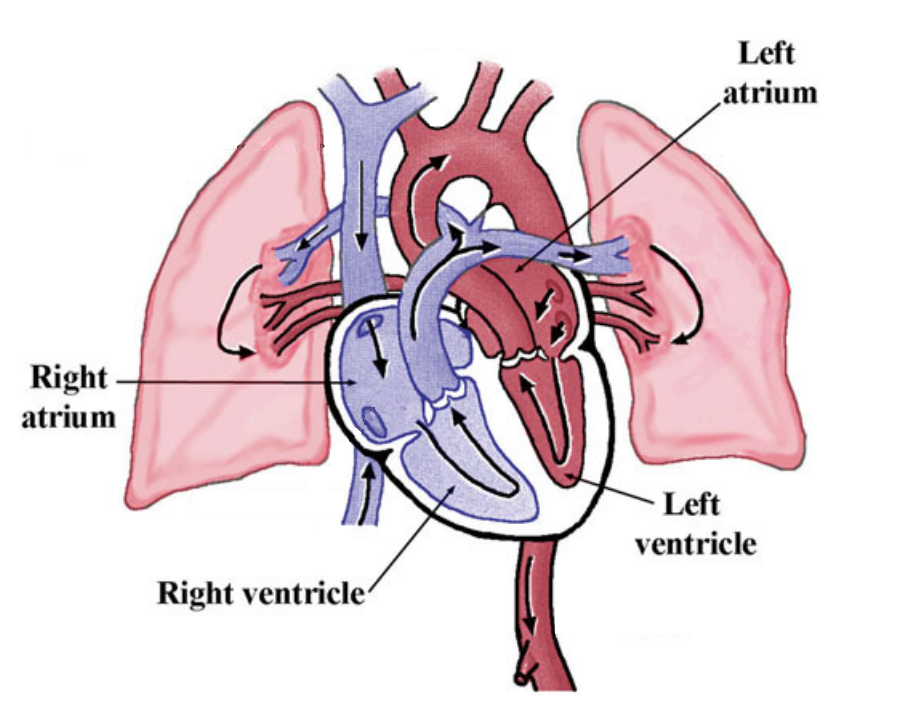
\includegraphics[width=0.5\textwidth]{images/BasicAnatomy.png}
    \caption{The anterior view of a simplified blood flow schematic of the heart and lungs. \citep{BasicAnatomy}}
        \label{fig2.1}
\end{SCfigure}
\begin{SCfigure}[0.5][h!]
    \centering
    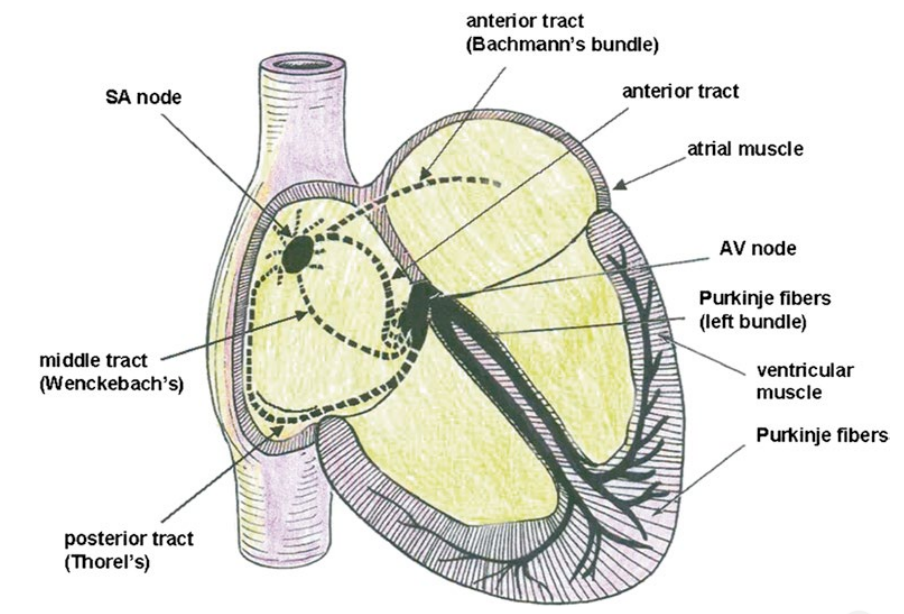
\includegraphics[width=0.7\textwidth]{images/ConductionSystem}
    \caption{Conduction System of the heart. The key areas of interest are the SA (sinoatrial) node and the AV (atrioventricular) node. Signals originate in the SA node and terminate in the muscular tissue via the Purkinje fibres. \citep{ConductionSystem}}
        \label{fig2.2}
\end{SCfigure}
The contracting phase of the cardiac cycle is known as systole, the relaxation phase where the ventricles refill is the diastole. The coordination of the millions of myocardial cells is required for effective pumping. This coordination is governed by the conduction system of the heart (see figure \ref{fig2.2}) and is achieved via electrical excitations, known as action potentials, which propagate through the heart's conductive cells thus activating the cardiac myocytes for muscular contractions. The action potentials of one cell conduct to the next via gap junctions (see section \ref{gapjunctions}). Originating from the sinoatrial node (SAN) in the right atrium, the signal propagates to the atrioventricular node (AVN) and then to to the ventricular muscle via the bundle of His and Purkinje fibres. \par

The main area of interest in this paper is the pacemaker function of the heart, this is controlled by the SAN-AVN complex. As such, the focus of the remainder of this section will be on the right atrium and the ventricular response of the heart will be largely ignored.

\subsection{Cardiac Electrophysiology}
The normal functioning of the heart is dependent on the coordinated contractions of the cardiac myocytes, the muscle cells within the heart. They function due to the charge difference across the membrane of the cell. This creates an electric potential known as the membrane potential. The contraction of the cells is stimulated by an action potential, a depolarizing transitory membrane potential, this interaction is explained in more depth in sections \ref{cellelectro} \& \ref{gapjunctions}. This stimulation originates from the SAN which acts as the pacemaker of the heart. \par

This extracellular potential can be measured using an electrocardiogram (ECG) which comprises of multiple electrodes placed at standardised positions on the body. A basic ECG can be acquired with three electrodes, known as the Einthoven leads, which are placed on the left arm $\Phi_L$, right arm $\Phi_R$, and the left foot $\Phi_F$. The potentials between these electrodes are known as Einthoven standard limb leads and are defined as
\begin{equation}
    \begin{split}
        & V_I = \Phi_L - \Phi_R \\
        & V_{II} = \Phi_F - \Phi_R \\
        & V_{III} = \Phi_F - \Phi_L
    \end{split}
    \label{Eq2.1}
\end{equation}
The Einthoven method assumes the heart is located at the centre of a homogeneous spherical conductor as shown in figure \ref{fig2.3}. Additional leads can be used to obtain more complete ECGs. These additional leads are known as augmented leads ($aV_R, aV_L, aV_F$), which bisect the Einthoven leads, and precordial leads ($V_1, ..., V_6$), which are placed at locations on the chest. The ECG that is typically seen is the voltage over time measured by lead I and is shown in figure \ref{fig2.3}.
\begin{figure}[H]
    \centering
    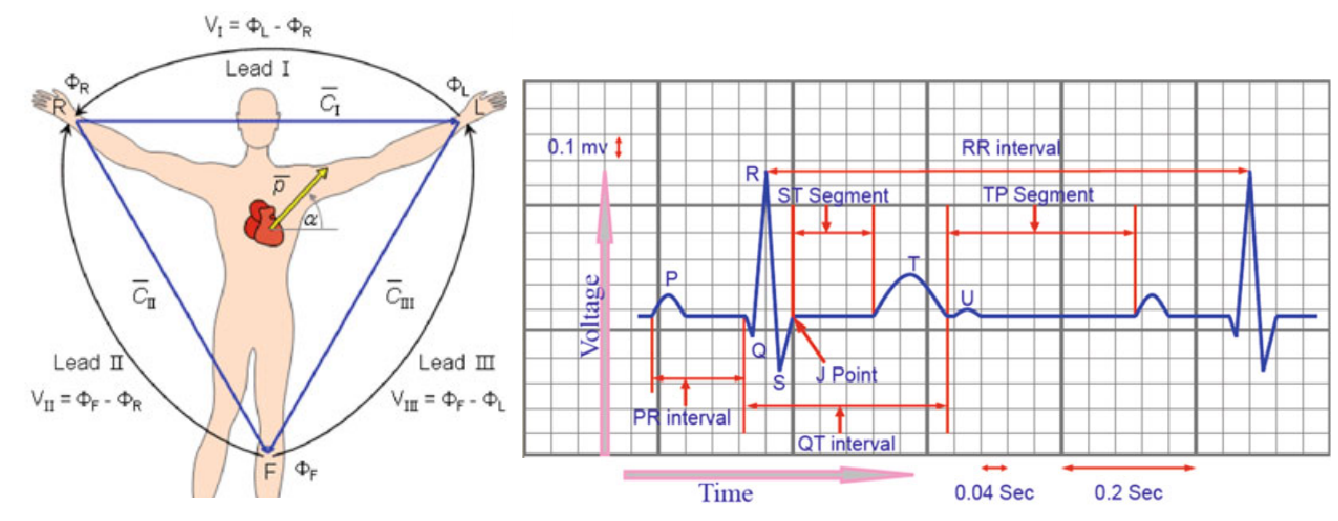
\includegraphics[width=1\textwidth]{images/ECGbasics.png}
    \caption{A Schematic view of Einthoven standard limb leads (left) and a schematic view of a normal lead I ECG (right). \citep{ecg}}
    \label{fig2.3}
\end{figure}
As can be seen in the lead I ECG, the voltage changes as the heart goes through a cardiac cycle. Each deflection from the resting potential corresponds to a different phase of the cycle. The P wave is associated with atrial depolarisation and is the main area of interest of this paper, the atrial repolarisation is obscured by the much larger QRS complex. The QRS complex corresponds to the ventricular contraction. The T wave is the result of the ventricular repolarisation. The relation of each deflection on an ECG with the cardiac cycle can be seen on a Wiggers diagram (figure \ref{fig2.4}).\par
\begin{figure}[H]
    \centering
    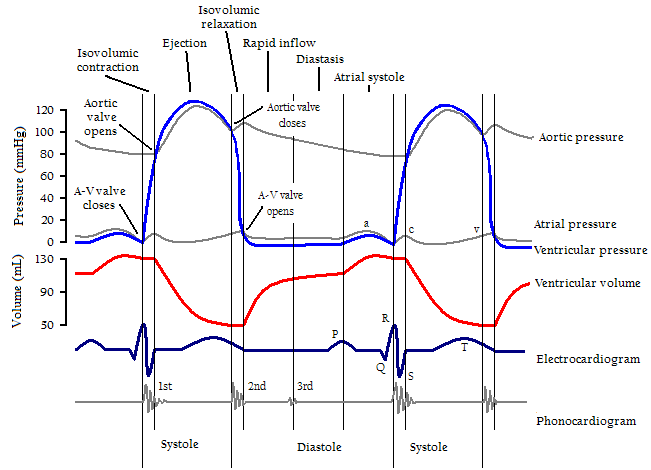
\includegraphics[width=0.95\textwidth]{images/Wiggers_Diagram.png}
    \caption{Wiggers diagram of a cardiac cycle. \citep{wiggers}}
    \label{fig2.4}
\end{figure}
The P wave is of particular interest in this paper as it can be thought of as the average action potential across the atria. The action potentials of the cells at various locations within the heart are different based on their function. For the P wave the cells of interest are nodal cells and the atrial conduction cells.

\subsection{Single Cardiac Cell Electrophysiology} \label{cellelectro}
Ventricular and atrial action potentials are controlled by voltage gated ion channels and can be described as a five phase process as shown in figure \ref{fig2.5}. \par
\begin{SCfigure}[0.5][h!]
    \centering
    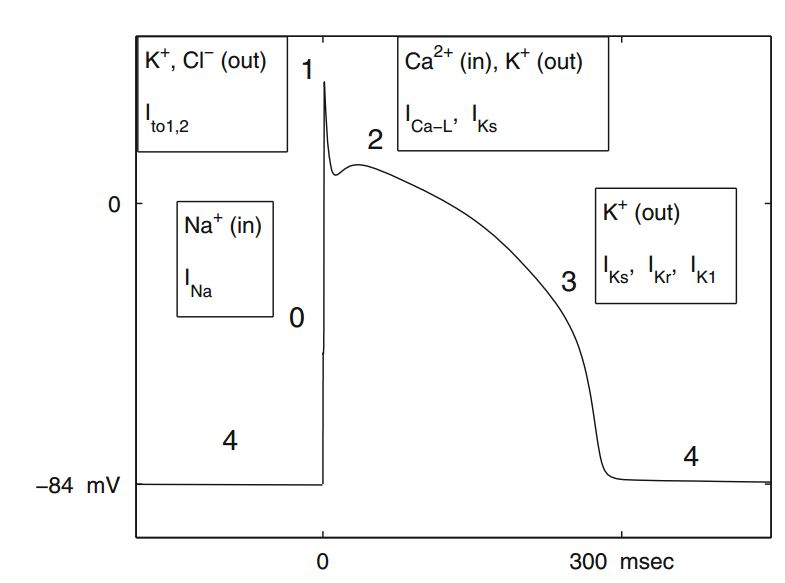
\includegraphics[width=0.7\textwidth]{images/actionpotential.png}
    \caption{Schematic plot of an atrial conduction cell action potential with phases 0 through 4. The ions associated with each phase are shown. \citep{ecg}}
    \label{fig2.5}
\end{SCfigure}
\textbf{Phase 0: Depolarisation.} Rapid depolarisation due to the opening of $Na^+$ channels and the rapid uptake of $Na^+$ by the cell. \par
\textbf{Phase 1: Peak.} The deactivation of the $Na^+$ channels and the release of $K^+$ \& $Cl^-$. \par
\textbf{Phase 2: Plateau.} A balanced flow of inward $Ca^{2+}$ and outward $K^+$. It is these calcium ion currents that cause the cardiac action potentials to have longer duration than neuronal action potentials. \par
\textbf{Phase 3: Repolarisation.} $Ca^{2+}$ channels close and more $K^+$ channels open. \par
\textbf{Phase 4: Resting.} The cell is restored to its resting potential until stimulated by an external source. \par
Nodal cells function slightly differently, these cells spontaneously rise to the threshold voltage of the $Ca^{2+}$ channels allowing them to autonomously activate. There is no phases 1 or 2 in nodal cells as the depolarisation is caused by comparatively slow $Ca^{2+}$ channels due to the lack of fast $Na^+$ channels in SAN cells. The opening of the voltage-gated $K^+$ channels cause the repolarisation phase 3. This reaches a minimum potential whereby the channels close and the cell slowly repolarises due to what are described as leaky $Na^+$ channels \citep{ConductionSystem}. Due to this spontaneous excitation, the SAN has the most rapid and regular excitation causing it to govern the heart rate via a principle known as overdrive suppression. In a normal healthy heart this excitation rate is between 60-100 beats/min. The conduction cells between the SA and AV node cells also have a degree of spontaneous excitation but at a slower rate than the nodal cells, meaning the nodes control excitation rate. A schematic of a nodal action potential can be seen in figure \ref{fig2.6}. \par
\begin{SCfigure}[0.95][h!]
    \centering
    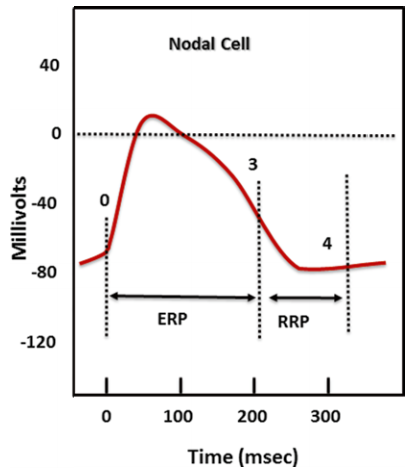
\includegraphics[width=0.4\textwidth]{images/nodalpotential.png}
    \caption{A schematic of the action potential of a nodal cell. Phases 1 and 2 are not observed. There is no stable resting potential. The refractory period for nodal cells is limited by the potential for opening $Ca^{2+}$ channels. \citep{ConductionSystem}}
    \label{fig2.6}
\end{SCfigure}
%push onto next page
\newpage
A typical cardiac conduction cell has a resting membrane potential ($V_m$) between -80 and -90 mV. This is found using the Goldman-Hodgkin-Katz (GHK) equation;
\begin{equation}
    V_m = (2.3R*T/F)*log_{10}\frac{P_K[K]_o + P_{Na}[Na]_o + P_{Cl}[Cl]_i + P_{Ca}[Ca]_i}{P_K[K]_i + P_{Na}[Na]_i + P_{Cl}[Cl]_o + P_{Ca}[Ca]_o}
    \label{eq2.2}
\end{equation}
where $P$ is the permeability, $[X]_x$ is the intracellular and extracellular concentrations of ion X, $T$ is the temperature, $R$ is the ideal gas constant and $F$ is Faraday's constant. The term for calcium, however, is regularly ignored due to the comparatively low concentrations of the ion, as shown in table \ref{table2.1}. When calculated with the GHK equation, typical values found for the resting potential lie around -84 mV. \par
\begin{table}[h!]
\centering
 \begin{tabular}{||c c c||} 
 \hline
 Ion & Intracellular Concentration (mM) & Extracellular Concentration (mM) \\ [0.5ex] 
 \hline\hline
 Na & 5-34 & 140 \\ 
 \hline
 K & 104-180 & 5.4 \\
 \hline
 Cl & 4.2 & 117 \\
 \hline
 Ca & - & 3 \\
 \hline
\end{tabular}
\caption{Typical resting ion concentrations for a typical cardiac cell. \citep{ionconc}}
\label{table2.1}
\end{table}
Individual cell types have slightly different observed properties which govern how the signal propagates through the heart. Table \ref{table2.2} and figure \ref{fig2.7} detail the action potentials of the cells of interest in this paper.
\begin{table}[h!]
\centering
 \begin{tabular}{||c c c c c c||} 
 \hline
 Cell & DP (mV) & Upstroke (mV/ms) & Peak (mV) & APD (ms) & PV (mm/ms) \\ [0.5ex] 
 \hline\hline
 SAN & -50,-60 & 1-10 & 30 & 100-200 & 0.03-0.05 \\ 
 \hline
 Atria & -80 & 100-200 & 30 & 100-200 & 0.3-0.7 \\
 \hline
 AVN & -60,-70 & 5-15 & 20 & 100-300 & 0.1 \\
 \hline
\end{tabular}
\caption{Average values of diastolic potential (DP), upstroke velocity (Upstroke), peak potential (Peak), action potential duration (APD) and propagation velocity (PV) for the cells of interest \citep{ecg}.}
\label{table2.2}
\end{table}
\begin{SCfigure}[0.9][h!]
    \centering
    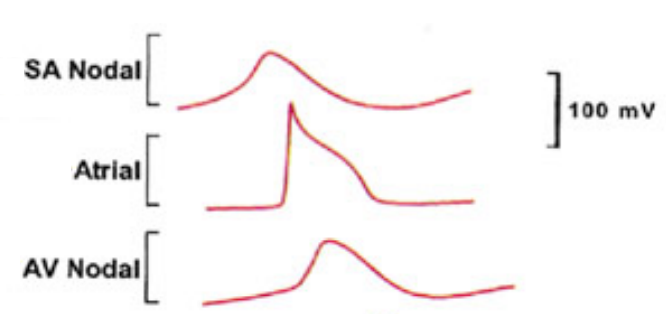
\includegraphics[width=0.4\textwidth]{images/cardiacactionpotentialregions.png}
    \caption{Schematic diagram of typical action potentials observed for the cells of interest. The duration of the potential is approximately 0.3 seconds. \citep{ecg}}
    \label{fig2.7}
\end{SCfigure}

\subsection{Gap Junctions \& Multiple Cells} \label{gapjunctions}
Cells are connected end to end by intercalated disks holding the cells together. Adjacent to these disks are gap junctions. Gap junctions allow action potentials to spread from one cell to the next via low-resistance pathways formed by protein connections on the disks \citep{gapjunctions}. It takes approximately 30 ms for excitation to spread between the SAN and AVN and activation occurs over 70-90 ms. Gap junctions are key factors in heart disease; issues with gap junctions have been linked to arrhythmia, ischemia and heart failure.\par

Gap junctions are more abundant in the connections between the ends of the cells than the sides allowing for faster propagation along a fibre than perpendicular to it, however, fibres in the atria are very irregular. Due to this anisotropy it is impractical to model gap junctions explicitly. Instead a continuum approach is usually used in mathematical models and the propagation between cells is described by diffusion of ions through a uniform space. More sophisticated models have described this propagation using 3 dimensional tensor mathematics \citep{unansweredquestions}. \par

One key observation to be made when considering activation propagation across multiple cells is that the action potential duration is much longer than the time taken to propagate across the atrium \citep{ecg}. The action potential lasts approximately 0.3 seconds but only 0.03 seconds for the excitation to spread between the SAN and AVN. This means that the whole medium is excited at the same time suggesting that it is the trailing edge of the wave front which causes re-entry in the presence of blockers.

\subsection{Refractory Periods \& Re-entry}
\label{section2.4}
An important property of individual cells is that they have a refractory period after excitation in which the cell recovers. One effect of this is to prevent rapid stimulation; if rapid stimulation occurred continuously the contraction ability of cells would be inhibited reducing cardiac output. This property prevents rapid stimulation propagating through the tissue, this has important effects on re-entry. \par

Re-entry is where a propagating wave is self-sustained in the tissue. This may occur as a spiral wave propagating around a blocker (see figure \ref{fig2.8}). The refractory period of cells helps prevent re-entry by not allowing cells to re-excite for a period of time, however, in the case of a uni-directional current block the wave can propagate around the block and then re-enter through the opposing side allowing enough time for cell recovery. Re-entry is a primary cause of many arrhythmias and has been linked to many cardiac diseases, understanding its effects are key to developing treatments. \par
\begin{figure}[h]
    \centering
    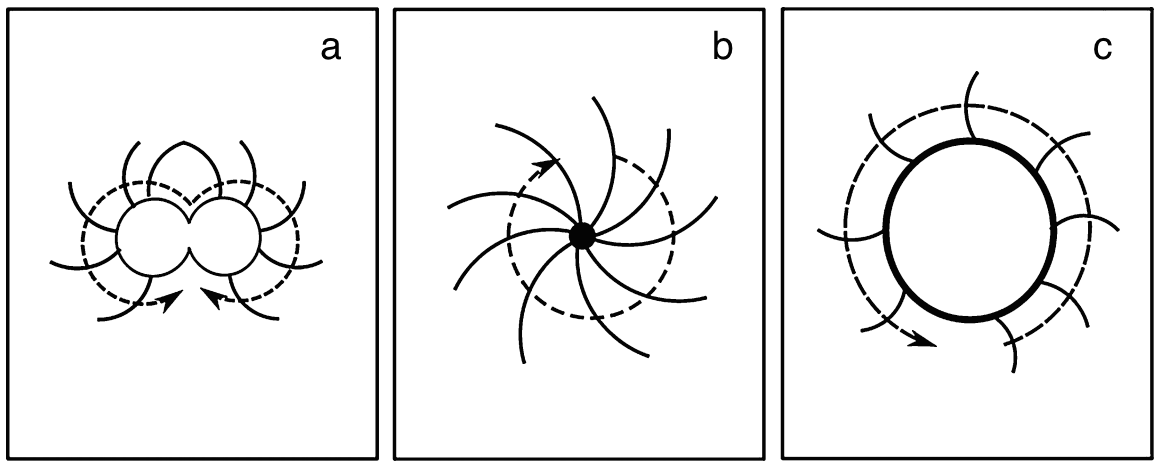
\includegraphics[width=0.9\textwidth]{images/reentry.png}
    \caption{Re-entry schematic. Dotted arrow shows wave propagation direction. (a) Shows two waves rotating in opposite directions around a blocker, if uni-directional the wave can back-propagate through the block. (b) Shows a spiral wave around a central node. (c) Shows a wave propagating around a large structural obstacle. \citep{phdpaper}}
    \label{fig2.8}
\end{figure}

\subsection{Cardiac Arrhythmias and Diseases}
Arrhythmias refer to either the lack of rhythm or irregular rhythm of the heart beat. Irregular contraction can lead to restricted output or even death. The majority of cardiac conditions are the result of, or lead to, arrhythmias. Bellow are some of the common arrhythmia related diseases.
\subsubsection{Tachycardia}
Tachycardia is the fast reactivation of the heart, resulting in a faster than normal resting heart rate. Commonly the result of re-entrant waves due to the presence of uni-directional blockers in the conductive tissue. Associated with reduced cardiac output and have a chance to develop into fibrillation.
\subsubsection{Bradycardia}
Bradycardia refers to the slow reactivation of the heart. Associated with atrioventricular nodal blocks and underlying problems with the heart rate regulatory system. Bradycardia results in reduced cardiac output significantly reducing nutrient and oxygen supply to organs.
\subsubsection{Ischemia}
Ischemia is the result of a portion of cell death within the heart tissue, an antisymmetric omni-directional block. These regions do not contract or pass conduction signals, resulting in reduced cardiac output. If of significant size this can block wave propagation resulting in re-entry potentially causing tachycardia and fibrillation.
\subsubsection{Fibrillation}
The fast and irregular activation of the heart is known as fibrillation. Associated with the re-entry of spiral waves, fibrillation has a serious effect on cardiac output and coordination. Atrial fibrillation can predispose ventricular fibrillation, commonly known as a heart attack, and death.
